\section{Experiments}
\label{sec:experiments}

\subsection{Setup}
\label{sec:setup}

\paragraph{Data and metric.}
We use the official SPair-71k splits: 53{,}340 training, 5{,}384 validation and 12{,}234 test pairs. Training uses only the training split. The validation split selects the training checkpoint, the WSA window and temperature, and the feature layer; the test split is evaluated once per configuration. We report PCK at $\alpha\in\{0.05,0.1,0.2\}$ relative to the target bounding box, measured in original image pixels. Unless stated otherwise PCK is averaged \emph{per image} (the mean over pairs of the fraction of correct keypoints), the convention of supervised methods~\cite{zhang2024telling}; per-keypoint averages are in the supplementary material (\cref{tab:main_pt}).

\paragraph{Training.}
All adapted models are trained with AdamW and the loss of \cref{eq:loss}, at a constant learning rate: $5\times10^{-5}$ with weight decay $0.01$ for fine-tuning, $10^{-3}$ without weight decay for LoRA, whose rank already constrains the update. The effective batch is 20 pairs for every backbone; for SAM it is obtained as two accumulated micro-batches of 10, which gives the same gradient because the loss is a mean over pairs and the backbones contain no batch-dependent layers. Training runs in bfloat16 autocast with similarity maps and loss in float32. Photometric augmentation (brightness, contrast and saturation in $[0.85,1.15]$, hue in $[-0.05,0.05]$, applied identically to both images with probability $0.9$) is used unless stated otherwise; geometric augmentation is excluded because it would require consistent keypoint remapping. We train for up to 50 epochs with early stopping on the validation loss (patience 7) and keep the checkpoint with the lowest validation loss. All 27 training runs and all evaluations were executed on single NVIDIA H100 NVL GPUs.

\subsection{Main results}
\label{sec:main_results}

\begin{table*}[t]
\centering
\caption{PCK (\%) on the SPair-71k test split, averaged per image. FT: fine-tuning of the last $N$ blocks; LoRA: rank-8 adapters on the MLPs of the last $N$ blocks; WSA: window soft-argmax with $(w,\tau)$ selected on the validation split. Bold: best per backbone and column.}
\label{tab:main}
\small
\begin{tabular}{llcr ccc ccc}
\toprule
 & & & Trainable & \multicolumn{3}{c}{Argmax} & \multicolumn{3}{c}{WSA} \\
\cmidrule(lr){5-7}\cmidrule(lr){8-10}
Backbone & Method & $N$ & params & @0.05 & @0.1 & @0.2 & @0.05 & @0.1 & @0.2 \\
\midrule
\multirow{7}{*}{DINOv2} & Frozen & -- & 0 & 36.8 & 53.2 & 68.4 & 37.7 & 55.3 & 69.7 \\
 & FT & 1 & 7.1M & 63.2 & 80.4 & 89.9 & 67.8 & 82.4 & 90.7 \\
 & FT & 2 & 14.2M & \textbf{67.6} & \textbf{83.4} & \textbf{91.1} & \textbf{71.7} & \textbf{84.9} & \textbf{91.8} \\
 & FT & 4 & 28.4M & 66.8 & 79.8 & 86.9 & 70.6 & 80.9 & 87.4 \\
 & LoRA & 1 & 61K & 53.8 & 71.6 & 83.5 & 58.2 & 74.3 & 84.5 \\
 & LoRA & 2 & 123K & 56.0 & 74.0 & 85.6 & 60.5 & 76.8 & 86.5 \\
 & LoRA & 4 & 246K & 61.6 & 77.4 & 85.9 & 66.4 & 79.2 & 86.4 \\
\midrule
\multirow{7}{*}{DINOv3} & Frozen & -- & 0 & 32.4 & 47.8 & 61.8 & 32.8 & 49.2 & 62.6 \\
 & FT & 1 & 7.1M & 57.3 & 77.1 & 88.3 & 62.6 & 79.1 & 88.8 \\
 & FT & 2 & 14.2M & 60.9 & \textbf{79.0} & \textbf{88.6} & 65.6 & \textbf{80.5} & \textbf{88.9} \\
 & FT & 4 & 28.4M & \textbf{62.8} & 78.3 & 86.9 & \textbf{67.3} & 79.4 & 87.1 \\
 & LoRA & 1 & 61K & 47.6 & 67.4 & 80.6 & 51.6 & 69.3 & 81.2 \\
 & LoRA & 2 & 123K & 53.9 & 73.5 & 85.4 & 59.2 & 75.4 & 85.8 \\
 & LoRA & 4 & 246K & 57.8 & 75.4 & 85.1 & 62.7 & 76.8 & 85.4 \\
\midrule
\multirow{7}{*}{SAM} & Frozen & -- & 0 & 14.1 & 22.2 & 35.5 & 13.5 & 22.7 & 35.9 \\
 & FT & 1 & 7.1M & 32.1 & 44.1 & 57.2 & 33.7 & 45.4 & 57.7 \\
 & FT & 2 & 14.2M & 31.1 & 43.6 & 56.2 & 33.2 & 44.7 & 56.4 \\
 & FT & 4 & 28.4M & \textbf{34.8} & \textbf{47.1} & \textbf{58.5} & \textbf{36.9} & \textbf{47.4} & \textbf{58.6} \\
 & LoRA & 1 & 61K & 29.5 & 40.3 & 54.0 & 30.5 & 42.0 & 54.7 \\
 & LoRA & 2 & 123K & 31.0 & 43.0 & 55.4 & 32.8 & 44.3 & 55.9 \\
 & LoRA & 4 & 246K & 32.4 & 44.3 & 56.2 & 34.4 & 45.4 & 56.5 \\
\bottomrule
\end{tabular}
\end{table*}


\Cref{tab:main} reports all configurations. Three observations hold for every backbone.

\emph{Adaptation dominates.} Every adapted model is far above its frozen counterpart: with WSA, the best fine-tuned model gains $29.6$ points of PCK@0.1 for DINOv2, $31.3$ for DINOv3 and $24.8$ for SAM. Fine-tuning two blocks is the best DINOv2 setting at every threshold; for DINOv3, $N{=}2$ is best at $\alpha\geq0.1$ and $N{=}4$ at $\alpha{=}0.05$; for SAM, $N{=}4$ is best throughout.

\emph{The backbone ranking is stable.} DINOv2 is ahead of DINOv3 in every cell of \cref{tab:main}, by $5.4$ points PCK@0.1 for the frozen models (argmax) and $4.4$ points for the best fine-tuned ones (WSA). SAM is far behind: even its best fine-tuned model ($47.4$) stays below frozen DINOv2 and $37.5$ points below the best DINOv2 model.

\emph{WSA is a free improvement for adapted models.} It raises PCK@0.05 by $3.8$ to $5.3$ points for every adapted DINO model and by $1.0$ to $2.1$ for SAM, and PCK@0.1 by $0.4$ to $2.8$. At $\alpha{=}0.2$ the gain of adapted models shrinks to at most one point, as expected from a refinement that moves predictions by less than a patch. On frozen features the gain at $\alpha{=}0.05$ is below one point, and negative for SAM ($-0.7$): the peaks of untrained similarity maps are broad, so averaging inside the window pulls the estimate towards neighbouring, less similar cells.

\subsection{Comparison with published and peer results}
\label{sec:comparison}

\begin{table}[t]
\centering
\caption{SPair-71k test PCK (\%, per image). Published methods use DINOv2 at $840^2$ (and SD at $960^2$); ours and the peer projects use $512$--$518^2$ inputs. $^\dagger$per-image values computed from the peer's per-pair results; $^\ddagger$WSA tuned on test pairs.}
\label{tab:comparison}
\small
\setlength{\tabcolsep}{4pt}
\begin{tabular}{lcc}
\toprule
Method & @0.05 & @0.1 \\
\midrule
\multicolumn{3}{l}{\emph{Training-free}} \\
DINOv2-B + NN~\cite{zhang2023tale,zhang2024telling} & 38.4 & 53.9 \\
SD + DINOv2~\cite{zhang2023tale} & 44.7 & 59.9 \\
GeoAware-SC zero-shot~\cite{zhang2024telling} & 49.1 & 65.4 \\
Ours, DINOv2 frozen & 36.8 & 53.2 \\
Ours, DINOv2 frozen + WSA & 37.7 & 55.3 \\
\midrule
\multicolumn{3}{l}{\emph{Supervised}} \\
SD + DINOv2, trained head~\cite{zhang2023tale} & 57.7 & 74.6 \\
GeoAware-SC~\cite{zhang2024telling} & 72.6 & 82.9 \\
GeoAware-SC, AP-10K pre-training~\cite{zhang2024telling} & 75.3 & 85.6 \\
Ours, DINOv2 FT $N{=}2$ + WSA & 71.7 & 84.9 \\
Ours, DINOv2 LoRA $N{=}4$ + WSA & 66.4 & 79.2 \\
\midrule
\multicolumn{3}{l}{\emph{Peer projects, best adapted model}} \\
P1~\cite{peer_tomm}: DINOv2 FT $N{=}2$ + WSA & 61.3 & 80.0 \\
P2~\cite{peer_parsa}: DINOv3 FT $N{=}2$ + WSA$^\dagger$ & 55.4 & 72.4 \\
P3~\cite{peer_hesam}: DINOv2 FT $N{=}1$ + WSA$^\ddagger$ & 53.9 & 69.1 \\
\bottomrule
\end{tabular}
\end{table}

\Cref{tab:comparison} places our models among published results and three independent implementations of the same course project. Our frozen DINOv2 matches the published nearest-neighbour baseline ($53.2$ vs.\ $53.9$ PCK@0.1 per image; $56.0$ vs.\ $55.6$ per keypoint~\cite{zhang2023tale}) despite a lower input resolution ($518$ vs.\ $840$). The frozen baselines of the peer projects agree with ours to within two points for every backbone (DINOv2 $51.9$--$52.5$, DINOv3 $48.2$--$48.3$, SAM $20.5$--$21.5$ PCK@0.1, against our $53.2$, $47.8$ and $22.2$), which independently confirms the evaluation protocol.

Our fine-tuned DINOv2 with WSA is on par with GeoAware-SC: two points above at $\alpha{=}0.1$, one point below at $\alpha{=}0.05$, and below its AP-10K pre-trained variant. GeoAware-SC keeps SD and DINOv2 frozen at higher resolution and trains a 5\,M-parameter head with geometry-aware augmentation, while we adapt the backbone itself at lower resolution, so the two results are complementary rather than directly competing. Among the peer projects, the closest setting (P1: DINOv2, two blocks, WSA) reaches $80.0$; P2 uses three epochs at learning rate $5\times10^{-6}$ with an effective batch of 4, and P3 a single fine-tuned block.

\subsection{Ablations}
\label{sec:ablations}

\begin{figure}[t]
    \centering
    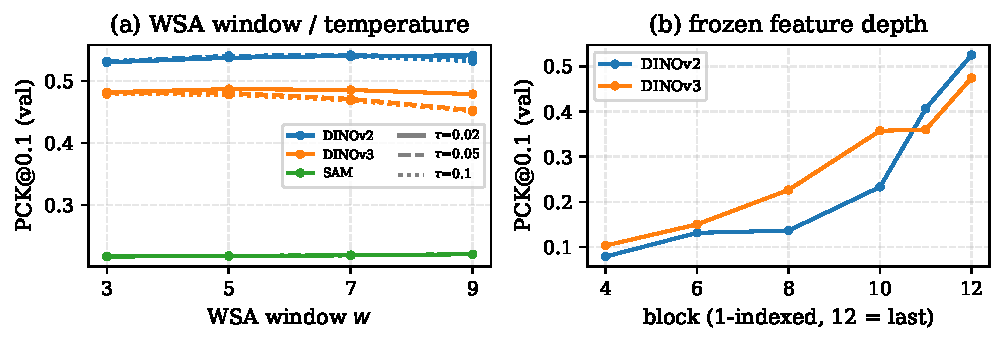
\includegraphics[width=\columnwidth]{img/sensitivity_combined.pdf}
    \caption{Inference choices on the validation split (frozen features). (a) PCK@0.1 with WSA as a function of the window $w$ and temperature $\tau$. (b) PCK@0.1 (argmax) of features taken from intermediate blocks; block 12 is the last.}
    \label{fig:sensitivity}
\end{figure}

\paragraph{Feature layer.}
\Cref{fig:sensitivity}b evaluates frozen DINO features from intermediate blocks on the validation split. Accuracy grows with depth for both backbones and is highest at the last block ($52.5$ PCK@0.1 for DINOv2, $47.4$ for DINOv3); block 4 reaches only $7.9$ and $10.3$. This agrees with~\cite{zhang2023tale}, who also use the last layer of DINOv2, and it is the only consistent choice for fine-tuning, which changes exactly the last blocks.

\paragraph{WSA window and temperature.}
On the validation split (\cref{fig:sensitivity}a) the selected settings are $(w,\tau)=(7,0.05)$ for DINOv2, $(5,0.02)$ for DINOv3 and $(9,0.05)$ for SAM. The surface is flat around the optimum: for the DINO models all windows from 3 to 9 at $\tau{=}0.02$ lie within $1.2$ points, while larger windows with a soft temperature lose accuracy for DINOv3, whose similarity maps have more secondary peaks. SAM varies by less than half a point.

\begin{figure}[t]
    \centering
    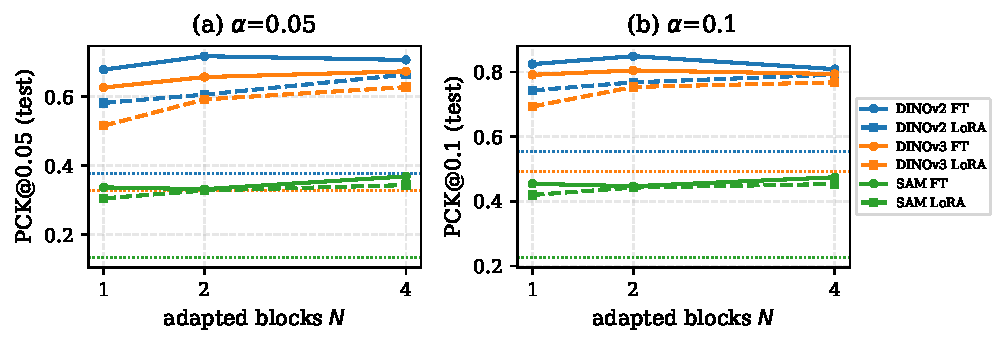
\includegraphics[width=\columnwidth]{img/depth_combined.pdf}
    \caption{Test PCK (with WSA) against the number of adapted blocks $N$ for fine-tuning (solid) and LoRA (dashed); dotted lines mark the frozen backbone with WSA.}
    \label{fig:depth}
\end{figure}

\paragraph{Adaptation depth and LoRA.}
\Cref{fig:depth} shows that LoRA improves monotonically with depth for all backbones and thresholds, whereas for the DINO models full fine-tuning gains little or loses beyond $N{=}2$ (DINOv2 loses $4.0$ PCK@0.1 from $N{=}2$ to $N{=}4$). The gap between the two shrinks accordingly: at $N{=}4$, LoRA recovers $93\%$ (DINOv2), $91\%$ (DINOv3) and $92\%$ (SAM) of the PCK@0.1 gain of fine-tuning the same blocks, with $246$K instead of $28.4$\,M trainable parameters. Against the best fine-tuning setting of each backbone, LoRA with $N{=}4$ still recovers $81\%$, $88\%$ and $92\%$ of the gain.

\begin{table}[t]
\centering
\caption{Photometric augmentation during fine-tuning: PCK@0.1 (\%, per image, WSA) on the SPair-71k test split.}
\label{tab:aug}
\small
\begin{tabular}{lcccc}
\toprule
Backbone & $N$ & with aug. & without & $\Delta$ \\
\midrule
DINOv2 & 1 & 82.4 & 82.3 & +0.1 \\
DINOv2 & 2 & 84.9 & 84.7 & +0.3 \\
DINOv2 & 4 & 80.9 & 81.3 & -0.4 \\
DINOv3 & 1 & 79.1 & 79.2 & -0.0 \\
DINOv3 & 2 & 80.5 & 80.5 & -0.0 \\
DINOv3 & 4 & 79.4 & 79.6 & -0.2 \\
SAM & 1 & 45.4 & 45.3 & +0.2 \\
SAM & 2 & 44.7 & 43.6 & +1.1 \\
SAM & 4 & 47.4 & 49.2 & -1.8 \\
\bottomrule
\end{tabular}
\end{table}


\paragraph{Photometric augmentation.}
Disabling augmentation (\cref{tab:aug}) changes PCK@0.1 by $-0.1$ points on average over the nine fine-tuning runs, and by at most $0.4$ points for the DINO models. Only SAM shows larger, opposite-signed differences ($+1.1$ at $N{=}2$, $-1.8$ at $N{=}4$), which we attribute to run-to-run variance: with a single seed per configuration, differences of this size are not significant. The mild colour jitter we use adds little variation beyond what the 53{,}340 training pairs already contain.

\subsection{Robustness and generalisation}
\label{sec:robustness}

\begin{figure}[t]
    \centering
    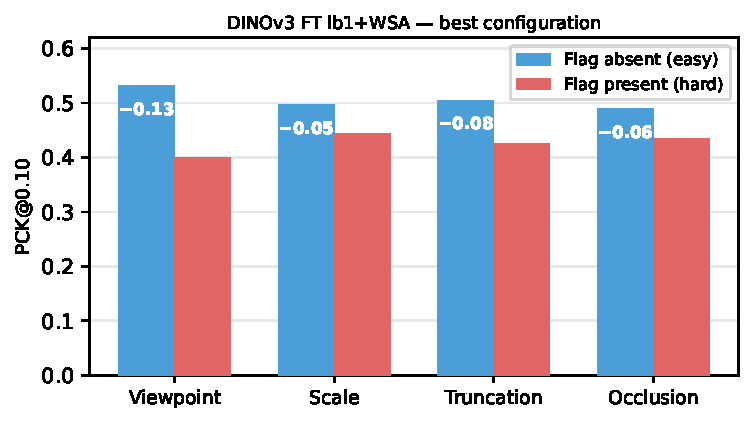
\includegraphics[width=0.92\columnwidth]{img/per_difficulty_a0.pdf}
    \caption{Test PCK@0.1 (WSA) of frozen and fine-tuned ($N{=}2$) DINOv2 on SPair-71k pairs with and without each difficulty flag.}
    \label{fig:per_difficulty}
\end{figure}

\paragraph{Difficulty factors.}
\Cref{fig:per_difficulty} splits the test pairs by the SPair-71k difficulty annotations. For the best model, truncation is the most harmful factor ($87.8$ vs.\ $81.0$ PCK@0.1), followed by occlusion ($85.8$ vs.\ $83.1$) and scale change ($86.2$ vs.\ $83.5$); pairs flagged for viewpoint change are not harder ($84.7$ vs.\ $85.1$). Fine-tuning improves every subset by 28--31 points, so it does not trade robustness for average accuracy.

\begin{table}[t]
\centering
\caption{PF-Willow: PCK (\%, per image, argmax) of SPair-71k models without retraining; threshold relative to the keypoint bounding box.}
\label{tab:pf_willow}
\small
\begin{tabular}{llcccc}
\toprule
Backbone & Method & $N$ & @0.05 & @0.1 & @0.2 \\
\midrule
DINOv2 & Frozen & -- & 40.2 & 66.4 & 89.3 \\
DINOv2 & FT & 1 & 53.6 & 78.1 & 95.1 \\
DINOv2 & FT & 2 & 54.0 & 77.9 & 94.8 \\
DINOv2 & FT & 4 & 55.5 & 78.1 & 94.4 \\
DINOv2 & LoRA & 1 & 48.0 & 72.5 & 92.4 \\
DINOv2 & LoRA & 2 & 50.2 & 74.7 & 93.2 \\
DINOv2 & LoRA & 4 & 52.1 & 76.9 & 93.1 \\
\midrule
DINOv3 & Frozen & -- & 44.1 & 72.2 & 91.8 \\
DINOv3 & FT & 1 & 52.5 & 78.0 & 94.8 \\
DINOv3 & FT & 2 & 53.9 & 79.8 & 94.9 \\
DINOv3 & FT & 4 & 53.8 & 78.6 & 94.4 \\
DINOv3 & LoRA & 1 & 47.8 & 75.9 & 93.4 \\
DINOv3 & LoRA & 2 & 49.0 & 75.4 & 93.4 \\
DINOv3 & LoRA & 4 & 51.4 & 76.4 & 93.1 \\
\midrule
SAM & Frozen & -- & 23.4 & 38.7 & 55.1 \\
SAM & FT & 1 & 32.2 & 49.3 & 65.6 \\
SAM & FT & 2 & 30.6 & 46.5 & 62.8 \\
SAM & FT & 4 & 30.7 & 48.9 & 62.4 \\
SAM & LoRA & 1 & 32.7 & 47.3 & 63.1 \\
SAM & LoRA & 2 & 29.0 & 43.7 & 58.7 \\
SAM & LoRA & 4 & 27.1 & 42.6 & 58.0 \\
\bottomrule
\end{tabular}
\end{table}

\begin{table}[t]
\centering
\caption{PF-Pascal: PCK (\%, per image, argmax) of SPair-71k models without retraining; threshold relative to the image size.}
\label{tab:pf_pascal}
\small
\begin{tabular}{llcccc}
\toprule
Backbone & Method & $N$ & @0.05 & @0.1 & @0.2 \\
\midrule
DINOv2 & Frozen & -- & 64.8 & 83.6 & 93.2 \\
DINOv2 & FT & 1 & 73.5 & 89.3 & 94.7 \\
DINOv2 & FT & 2 & 75.4 & 89.7 & 96.1 \\
DINOv2 & FT & 4 & 72.6 & 87.3 & 94.2 \\
DINOv2 & LoRA & 1 & 69.4 & 85.5 & 93.5 \\
DINOv2 & LoRA & 2 & 68.4 & 85.9 & 94.1 \\
DINOv2 & LoRA & 4 & 70.2 & 86.6 & 94.0 \\
\midrule
DINOv3 & Frozen & -- & 68.5 & 88.2 & 95.7 \\
DINOv3 & FT & 1 & 74.0 & 88.2 & 94.6 \\
DINOv3 & FT & 2 & 73.6 & 87.8 & 94.8 \\
DINOv3 & FT & 4 & 71.8 & 86.5 & 93.9 \\
DINOv3 & LoRA & 1 & 66.2 & 84.9 & 92.8 \\
DINOv3 & LoRA & 2 & 71.6 & 86.4 & 94.2 \\
DINOv3 & LoRA & 4 & 69.6 & 83.8 & 92.7 \\
\midrule
SAM & Frozen & -- & 30.2 & 44.1 & 61.9 \\
SAM & FT & 1 & 37.8 & 52.0 & 65.7 \\
SAM & FT & 2 & 34.7 & 47.2 & 63.4 \\
SAM & FT & 4 & 36.0 & 49.3 & 62.9 \\
SAM & LoRA & 1 & 35.9 & 49.4 & 65.0 \\
SAM & LoRA & 2 & 33.5 & 46.3 & 63.1 \\
SAM & LoRA & 4 & 33.1 & 46.7 & 62.6 \\
\bottomrule
\end{tabular}
\end{table}


\paragraph{Cross-dataset transfer.}
\Cref{tab:pf_willow} evaluates the SPair-71k models on the 900 PF-Willow test pairs without retraining. Every adapted model improves on its frozen backbone, \eg DINOv2 from $66.4$ to $77.9$ PCK@0.1 with two fine-tuned blocks, so the adaptation does not overfit to SPair-71k. The margins are smaller than on SPair-71k, and the DINOv2/DINOv3 ranking is reversed for the frozen models ($66.4$ vs.\ $72.2$); after fine-tuning the two backbones are within two points. PF-Willow has only four object classes and small pose changes, so these differences are less reliable than the SPair-71k ones.

On the 299 PF-Pascal test pairs (\cref{tab:pf_pascal}, threshold relative to the image size), fine-tuning again helps DINOv2 ($83.6\to89.7$ PCK@0.1 with $N{=}2$) and SAM ($44.1\to52.0$ with $N{=}1$). For DINOv3 it improves only the strict threshold ($68.5\to74.0$ PCK@0.05 with $N{=}1$), while at $\alpha{=}0.1$ no adapted model exceeds the frozen one ($88.2$). With a threshold relative to the whole image, PF-Pascal leaves little room above strong frozen features, and its 299 pairs make differences of one point uncertain.

\subsection{Qualitative results}
\label{sec:qualitative}

\begin{figure*}[t]
    \centering
    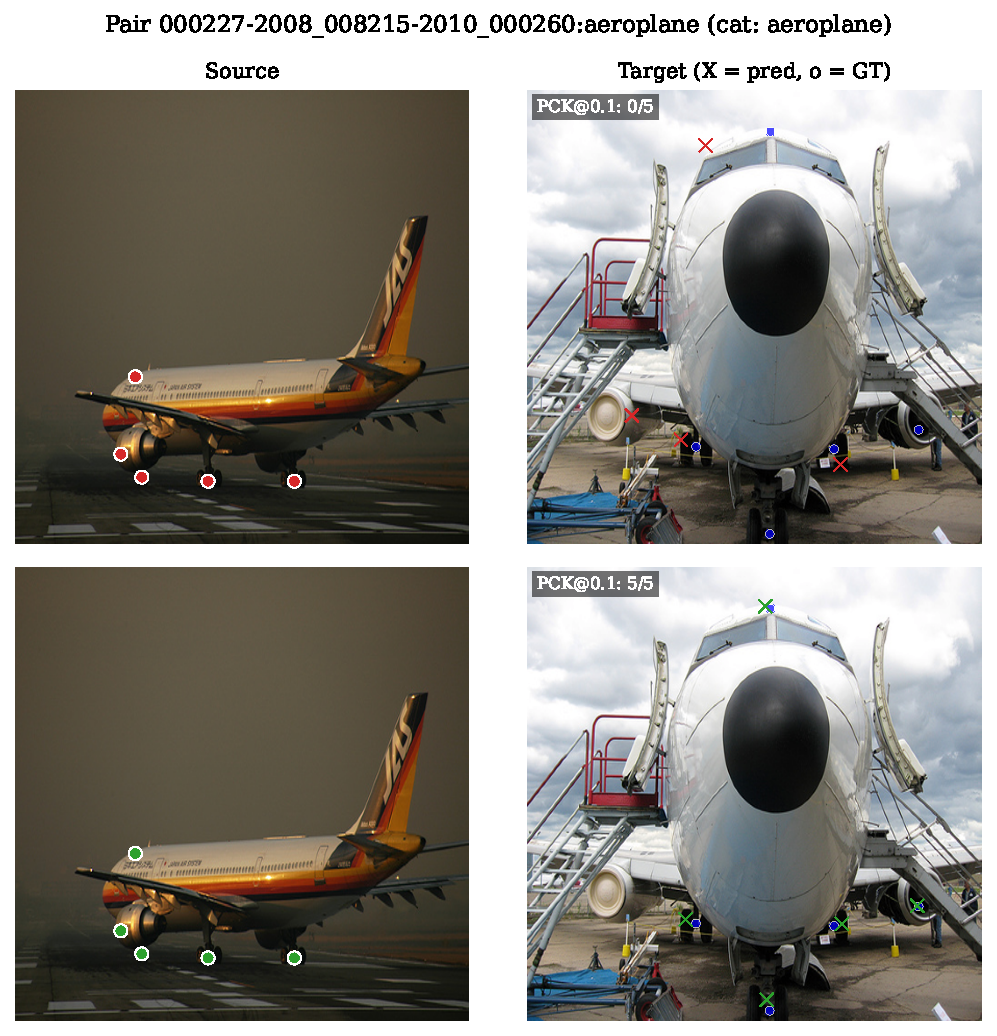
\includegraphics[width=0.325\textwidth]{img/qual_218.pdf}\hfill
    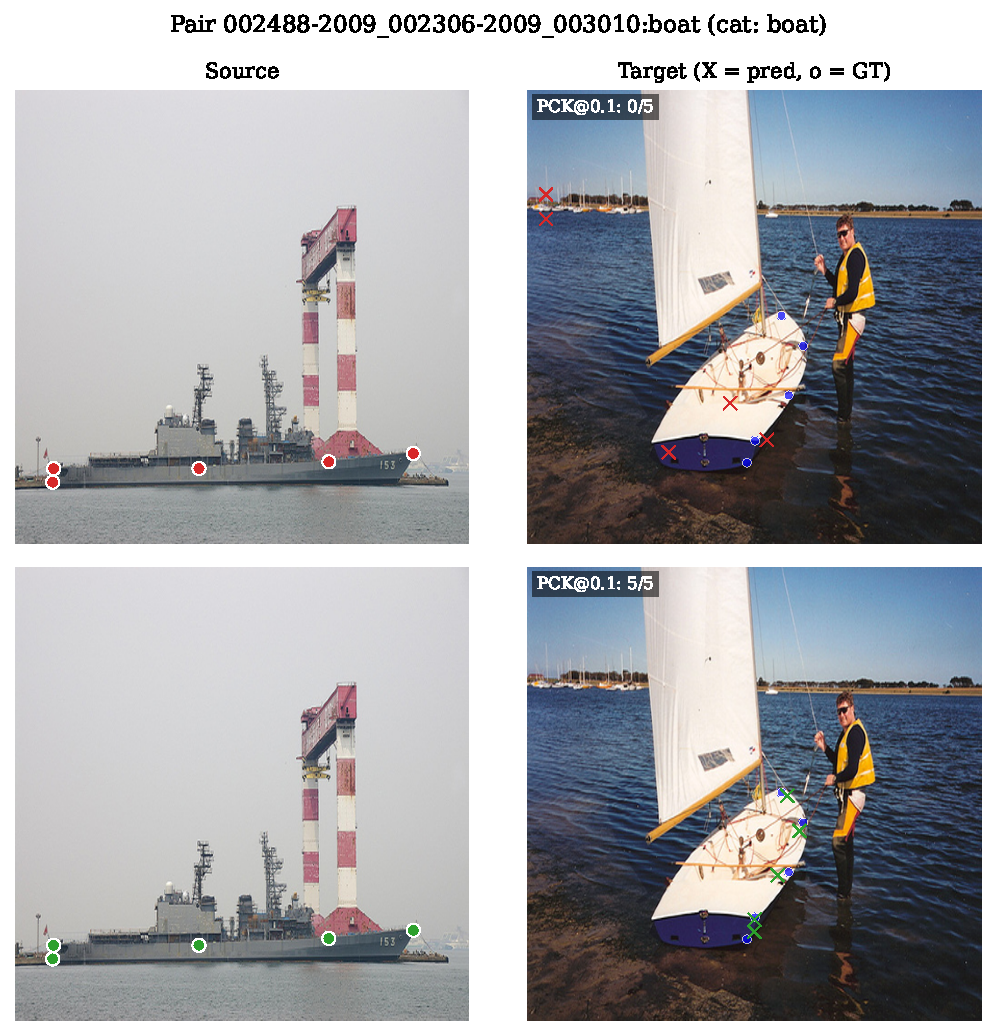
\includegraphics[width=0.325\textwidth]{img/qual_2394.pdf}\hfill
    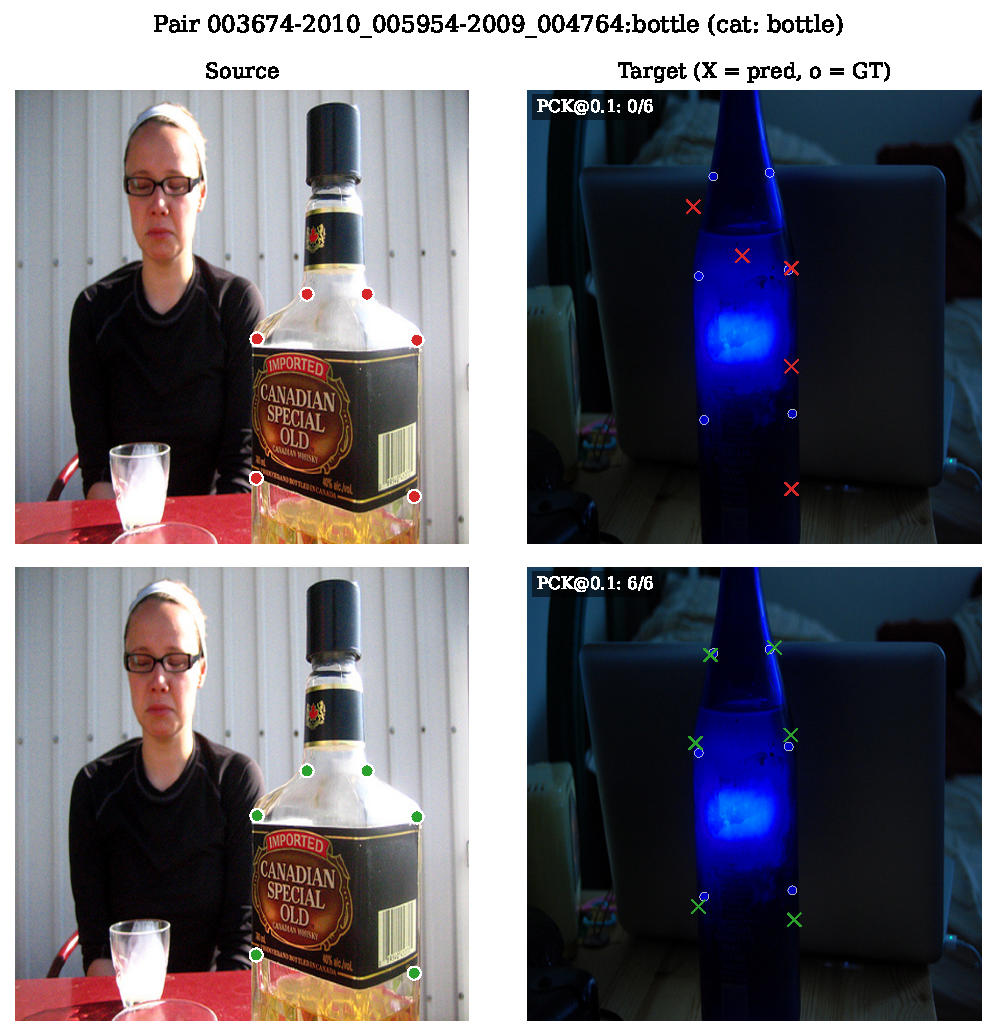
\includegraphics[width=0.325\textwidth]{img/qual_3540.pdf}
    \caption{DINOv2 predictions on SPair-71k test pairs, frozen with argmax (top row of each panel) and fine-tuned with $N{=}2$ and WSA (bottom). Source keypoints are green if matched correctly at $\alpha{=}0.1$ and red otherwise; in the target, crosses are predictions and dots ground truth. The pairs were selected as those with the largest per-image gain from fine-tuning, one per category, so they illustrate the kind of error that adaptation fixes, not typical accuracy.}
    \label{fig:qualitative}
\end{figure*}

\Cref{fig:qualitative} shows the failure modes of frozen features that fine-tuning removes. Under strong viewpoint change (aeroplane seen from behind and from the front, warship and dinghy), frozen DINOv2 matches parts to the wrong side of the object or to the background; under a large change of appearance (clear bottle in daylight, blue backlit bottle) it falls back to texture. The fine-tuned model places every keypoint on the corresponding part.

